\subsubsection{Devices}

Devices will be detailed separarely between read-only, toggleable and adjustable ones.

\subsubsection{Thermometer}

The thermometer is modelled as an extension of \texttt{Device} since it's not meant to be controllable
but only to return a \texttt{DeviceState} to the Controller,
and \texttt{DiscreteObject}, to define how should the temperature be sensed (in
a simple case, it could be updated directly, or in another case imperfections such as lag can be modelled).

% The DiscreteObject could also have been directly implemented instead of being extended by Thermometer,
% but I wanted to put 

\begin{figure}[H]
\centering{}
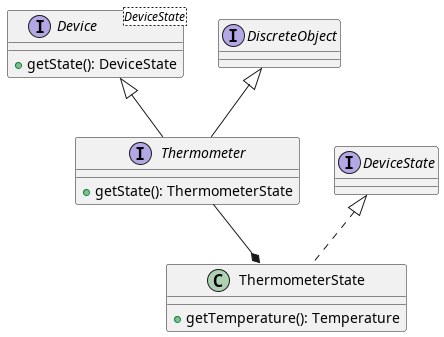
\includegraphics[width=\textwidth,height=\textheight,keepaspectratio]{magnani/uml/thermometer.png}
\caption{UML diagram of the thermometer}
\label{magnani:uml:thermometer}
\end{figure}

\paragraph{Problem} There are multiple devices that need to interact with a common temperature
\paragraph{Solution} Creation of the concept of \texttt{Environment} which represents the
physical simulated environment with its temperature parameter.
In the future, this would also allow to simulate different environments, eg. different rooms or completely
separate buildings.

\begin{figure}[H]
\centering{}
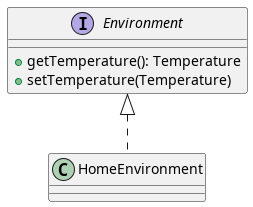
\includegraphics[keepaspectratio]{magnani/uml/environment.png}
\caption{UML diagram of the environment}
\label{magnani:uml:environment}
\end{figure}

\subsubsection{Lock}

The Lock has been modelled as a \texttt{ToggleableDevice}.
Its logic is really simple, the state can vary between locked and unlocked.
The lock is represented in figure \Cref{magnani:uml:lock}

\begin{figure}[H]
\centering{}
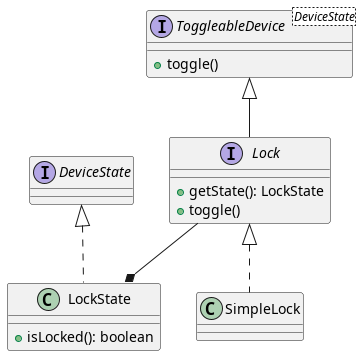
\includegraphics[width=10cm,height=\textheight,keepaspectratio]{magnani/uml/lock.png}
\caption{UML diagram of the lock}
\label{magnani:uml:lock}
\end{figure}

\subsubsection{Window, Door, Blinds}

The devices of type \texttt{Window, Door and Blinds} are modelled as \texttt{AdjustableDevice}s.

\paragraph{Problem} Each of these devices can be considered to be controllable between a range of values. Also, if those devices
were meant to be remotely controllable, there should be something that moves them.
\paragraph{Solution} Create the concept of \texttt{Actuator}. This also allows someone to decide however they want to model
the movement mechanism (as simplistically or realistically as preferred) $=>$ \texttt{Strategy} pattern.
It also allows to compartmentalize away the logic of the movement, adhering to the single responsibility principle.

\paragraph{Problem} Min, max values for ranges (eg. actuator movement range) require to be managed
in several parts. It is also necessary to make sure that the order of the values is correct.
This would lead to a lot of duplicated code.
\paragraph{Solution} Create a \texttt{Bounds} class encapsulating the concept of boundaries,
which also allows to check the correct order of the bounds internally.

\begin{figure}[H]
\centering{}
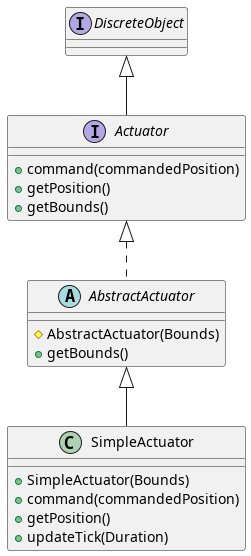
\includegraphics[width=\textwidth,height=12cm,keepaspectratio]{magnani/uml/actuator.png}
\caption{UML diagram of the actuator}
\label{magnani:uml:actuator}
\end{figure}

\paragraph{Problem} Reuse of code for the different devices.
\paragraph{Solution} Create the concept of \texttt{ActuatedDevice}. Then, create an \texttt{AbstractActuatedDevice}
which wraps an \texttt{Actuator} (\texttt{Decorator} pattern).
It is then possible to create several different implementations and choose which actuator implementation to use,
without having to create other device implementations that would be practically identical.

% Problem: Actuator in MechanizedWindow (we might want to change it eg. use a more realistic one)
% Solution: pass the actuator in the constructor, this allows to use different actuators without having
% to create other Window implementations that would only be different in terms of which actuator is being used.

\begin{figure}[H]
\centering{}
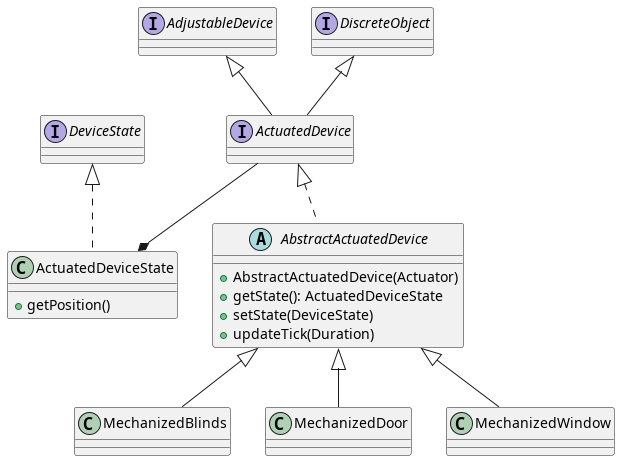
\includegraphics[width=\textwidth,height=\textheight,keepaspectratio]{magnani/uml/actuateddevice.png}
\caption{UML diagram of the ActuatedDevice and how the devices derive from it}
\label{magnani:uml:actuateddevice}
\end{figure}
